\section{第5讲\quad 综合}

\item {
    【逻辑推理】
    四百米比赛进入冲刺阶段,甲在乙前面30米,丙在丁后面60米,乙在丙前面20米. 这时,跑在前面的两位同学相差 \underline{\hbox to 20mm{}} 米.
    \vspace{1cm}
    % 2012华, 10
}

\item {
    老虎、狐狸、猴子各3只分别入住右图的9个房间中, 每个房间一只, 结果每只动物都说``有老虎与我相邻''(有公共边的两个房间相邻); 如果老虎都说真话, 狐狸都说假话, 猴子说的话不知真假, 那么说真话的猴子所在房间编号的和是\underline{\hbox to 20mm{}}.
    \begin{figure}[H] 
        \centering
        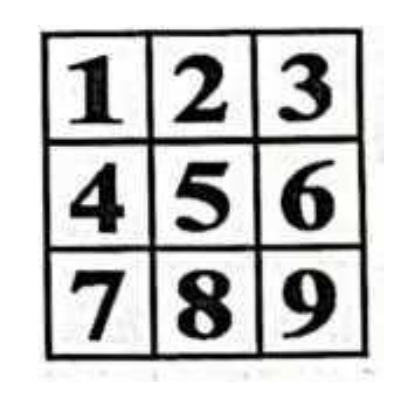
\includegraphics[width=0.3\textwidth]{./pics/Chapter_7/4.png}
    \end{figure}
    \vspace{1cm}
    % 2023; 15
}

\item {
    如图是一个棋盘, 开始时, 警察在位置A, 小偷在位置B. 双方交替走棋, 警察先走, 每次必须沿着线走一步. 那么警察至少需要走\underline{\hbox to 20mm{}}步才能保证抓住小偷.
    \begin{figure}[H] 
        \centering
        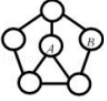
\includegraphics[width=0.3\textwidth]{./pics/Chapter_7/2015_1.png}
    \end{figure}
    \vspace{1cm}
    % 2015年“迎春杯”数学花园探秘科普活动试卷(小中组决赛c卷).doc; 4
}

\item {
    图1是由2个小等边三角形组成的菱形纸片; 图2是一个固定好的正六边形棋盘ABCDEF, 它由24个同样大小的小等边三角形组成, 现用12块菱形纸片完全覆盖正六边形棋盘, 共有\underline{\hbox to 20mm{}}种不同的覆盖方法.
    \begin{figure}[H] 
        \centering
        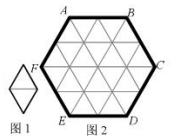
\includegraphics[width=0.3\textwidth]{./pics/Chapter_7/2015_2.png}
    \end{figure}
    \vspace{1cm}
    % 2015年“迎春杯”数学花园探秘科普活动试卷(小中组决赛b卷).doc; 20
}

\item {
    甲、乙、丙、丁四位绝世高手相约于华山之年比武论剑, 争夺 ``天下第一'' 的名号. 四人抽签两两分组各自决出胜者, 两位胜者再次比试决出一二名, 两位败者决出三四名. 比武结束后四人进行了交流, 每人说了两句话:\\
    甲: 我在与丙的大战中获得了胜利, 但是成输给了丁.\\
    乙: 我作为天下第一实至名归, 甲的名次比丙靠后.\\
    丙: 我被甲的六脉神剑击败了。乙在比试中输给了丁.\\
    丁: 好在我的名次没有垫底. 丙的名次比乙靠前.\\
    己知每个人在比试中胜了几场就说几句真话. 那么甲乙丙丁最终的名次按顺序组成的四位数为\underline{\hbox to 20mm{}}.
    \vspace{1cm}
    % 2022; 
}

\item {
    在算式 $\overline{A0AA}= A\times B\times \overline{BBA}$中, A、B 分别代表不同的数字.那么,  $\overline{AB}$ 代表的两位数是\underline{\hbox to 20mm{}}.
    \vspace{1cm}
    % 2022; 73
}

\item {
    如图所示, 正五边形的五个顶点位置分别标记为$1\sim 5$, 甲乙丙戊分别站在了这五个不同的顶点上, 发生如下对话:\\
    甲对乙说:我所在位置上的数比你大. \\
    乙对丙说:我所在位置上的数比你小. \\
    丙对丁说:我所在位置上的数比你大. \\
    丁对戊说:我所在位置上的数比你小. \\
    戊对甲说:我所在位置上的数比你大. \\
    如果五个人说的都是真话, 且任意发生对话的两个人都不相邻. 那么甲乙丙丁戊所站位置按顺序连成的五位数是\underline{\hbox to 20mm{}}.
    \vspace{1cm}
    % 2022; 31425
}

\item {
    甲、乙二人按如下顺序填写下图中的减法算式:\\
    $\textcircled{1}$甲选择一个数字, 然后乙选择一个位置将这个数字填入;\\
    $\textcircled{2}$甲选择一个之前没有选择过的数字, 然后乙选择一个位置将这个数字填入;\\
    $\textcircled{3}$甲选择一个之前没有选择过的数字, 然后乙将它填入最后一个位置;\\
    如果甲希望两个数的差尽量大, 乙希望这两个数的差尽量小, 那么甲、乙都按照最佳策略填写算式时, 差是\underline{\hbox to 20mm{}}.
    \zihao{3}
    \[
    \begin{array}{l@{\hspace{1em}} c@{\hspace{1em}} c@{\hspace{1em}} c@{\hspace{1em}} c@{\hspace{1em}}}
    & 2 & 0 & \square & \square \\
    - & & 2 & 2 & \square \\ 
    \hline
    \end{array}
    \]
    % \begin{figure}[H] 
    %     \centering
    %     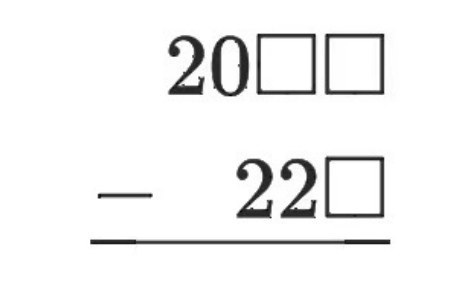
\includegraphics[width=0.2\textwidth]{./pics/Chapter_7/11.png}
    % \end{figure}
    \vspace{1cm}
    % 2022; 1854
}

\item {
    甲乙丙丁四个人各有一些糖果, 他们之间的对话如下:\\
    甲: 如果把我的糖果数量变成和丙一样多, 我们4人的平均数会减少2;\\
    乙: 如果我的糖果数量变成和丁一样多, 我们4人的平均数会减半; \\
    丙: 如果我的糖果数量变为原来2倍, 而甲的数量减半, 我们4人的平均数会增加 2; \\
    丁: 如果我的糖果数量变为原来2倍, 而乙的数量减半, 我们4人的平均数恰好会是一个整十数. \\
    事实证明, 他们4人中只有糖果数量最少的人说了假话, 并且糖果最多人的糖果数恰好是糖果最少人糖果数的3倍.那么, 他们4人一共有\underline{\hbox to 20mm{}}颗糖果.
    \vspace{1cm}
    % 2021; 120
}

\item {
    甲、乙、丙、丁共有糖果 17颗, 且每人的糖果数都不超过9颗. 他们有如下的对话:\\
    甲对乙说:``如果我给你1颗糖, 我们的糖果数就相同了.''\\
    乙对甲说:``如果你给我2颗糖, 我的糖果数就是你的3倍了.''\\
    丙对甲说:``如果我给你3颗糖, 你的糖果数就是我的3倍了.''\\
    丁对甲说:``如果你给我4颗糖, 我的糖果数就是你的4倍了.''\\
    结果发现:糖果数是奇数的人说的都是对的, 而糖果数是偶数的人说的都是错的.设甲、乙、丙、丁依次拥有 A、B、C、D颗, 那么, 四位数$\overline{ABCD}$是\underline{\hbox to 20mm{}}.
    \vspace{1cm}
    % 2021; 3158
}

\item {
    【综合·推理】现在有一台奇怪的电脑, 电脑上有个按键, 如果电脑上原来的数是3的倍数, 按下键后就会除以3; 如果电脑上原来的数不是3的倍数, 那么按下键后就会乘以6. 小明在按键前没有看屏幕上的数, 结果连按6次, 最后电脑上显示的数是12, 那么电脑上最开始的数最小可能是\underline{\hbox to 20mm{}}.
    \vspace{1cm}
}

\item {
    【综合·同余·周期】
    一条圆形跑道长 600 米,因铺设水管, 其中跑道上 AB 一段被挖开, 形成一个大坑. AB的跑道长度为 150 米.  有一机器人放在跑道上循环行走,  前进的步长(跑道弧长)为 d米, 可调整步长 d的大小,但调后不再改变,并且 d小于 600 米.请设计出两种(d 的不同长度)方案, 使得机器人不断循环, 并且永远不会落入坑里(碰到 A或 B也算落入坑里)每种方案包括:\\
    (1)步长d的值(不同方案的d的值). \\
    (2)机器人的出发点.
    \vspace{1cm}
    % 方案一:作一弧长 300米,该弧包含 AB,(4,B不在弧的端点上).机器人从该段弧的端点出发, d=300
    % 方案二:作一弧长 200 米, 该弧包含 AB,(A,B不在弧的端点上).机器人从该段弧的端点出发, d=200
    % 方案三:作一弧长 400米, 该弧的一半部分包含 AB,(4,B不在弧的端点与中点上).机器人从该段弧的端点出发, d=200.
    % 2021“华数之星”复评(初级)参考答案及评阅标准.pdf
}


\item {
    现有A、B、C、D、E五名诚实的安保在2016年12月1日~5日各值班三天, 每天将有3名安保值班, 每位安保值班安排5天一循环. 今天(2017年1月1日周日), 关于他们在上个月的值班情况, 5人进行了如下对话: \\
    A: 我和B在周末(周六、周日)值班的日子比其他3人都多; \\
    B: 我与其余4人在这个月都一起值过班; \\
    C: 12月3日本来我休息, 但那天恰逢数学花园探秘初赛, 于是我也来帮忙, 可惜不算值班; \\
    D: E每次都和我安排在一起; \\
    E: 圣诞节(12月25日)那天我和A都值班了. \\
    那么, 安保A在12月份中第2次、第6次、第10次值班日期顺次排列组成的五位数是\underline{\hbox to 20mm{}}.
    \vspace{1cm}
    % 2017年“迎春杯”数学花园探秘科普活动试卷(小中组决赛a卷).doc; 41016 
}

\item {
    在空格内填入数字$1\sim 6$, 使得每行、每列和每个粗线围成的区域里数字都是$1\sim 6$恰好各一个. 表外面的数字表示该行或该列的最近两个数的和. 那么, 第二列前四个数字按从上到下的顺序依次组成的四位数是\underline{\hbox to 20mm{}}.
    \begin{figure}[H] 
        \centering
        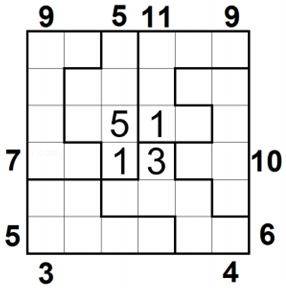
\includegraphics[width=0.4\textwidth]{./pics/Chapter_7/2016_1.png}
    \end{figure}
    \vspace{1cm}
    % 2016年“迎春杯”数学花园探秘网试试卷(四年级).doc; 1462
}

\item {
    如图, 有编号$1\sim 9$的9个小正方形狗舍, 每个狗舍至多住1只小狗; 原有3只小狗, 它们所在的狗舍互不相邻(相邻的小正方形有公共边); 当有新的小狗入住时, 与之相邻的小狗就会喊一声表示欢迎; 现在又先后依次新入住5只小狗, 每只小狗入住时都恰好有2只小狗喊一声; 已知第1只新入住的小狗住2号狗舍, 第2只新入住的小狗喊了2声. 第4只新入住的小狗住4号狗舍, 它没喊过; 就这5只新入住小狗所住狗舍号依次为A、B、C、D、E, 那么五位数$ABCDE=$\underline{\hbox to 20mm{}}.
    \begin{figure}[H] 
        \centering
        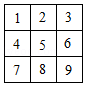
\includegraphics[width=0.2\textwidth]{./pics/Chapter_7/2016_2.png}
    \end{figure}
    \vspace{1cm}
    % 2016年“迎春杯”数学花园探秘决赛试卷(小中组c卷).doc; 25649
}

\item {
    甲乙两人轮流从$1\sim 9$这9个自然数中取不同的数, 对方取过的数不能再取, 谁取得的数中先有三个数成等差数列谁就获胜; 甲先取了8, 乙接着取了5; 为了确保甲必胜, 甲接下来取的一个数的所有可能值的乘积是\underline{\hbox to 20mm{}}.
    \vspace{1cm}
    % 2016年“迎春杯”数学花园探秘决赛试卷(小中组a卷).doc; 168
}

\item {
    甲、乙、丙、丁、戊五位同学在某次数学竞赛中获得了前5名(无并列), 照相时站成一排, 他们如下各说了一句话. \\
    甲说: 与我相邻的2位同学的名次都比我靠后; \\
    乙说: 与我相邻的2位同学的名次都与我的名次相邻; \\
    丙说: 我右边的所有同学(至少1位)的名次都比我靠前; \\
    丁说: 我左边的所有同学(至少1位)的名次都比我靠后; \\
    戊说: 我站在右数第2位. \\
    已知他们都是诚实的孩子, 甲、乙、丙、丁、戊分别获得第A、B、C、D、E名, 那么五位数$\overline{ABCDE}$是\underline{\hbox to 20mm{}}.
    \vspace{1cm}
    % 2016年“迎春杯”数学花园探秘初赛试卷(四年级d卷).doc; 23514 
}

\item {
    俊俊在看一个错误的一位数乘法算式, $A\times B=\overline{CD}$ (其中A、B、C、D所表示的数字互不相同), 聪明的俊俊发现, 如果只改动其中一个数字, 有3种方法可以将它改对; 如果只改变A、B、C、D的顺序, 也可以将它改对, 那么$A+B+C+D=$\underline{\hbox to 20mm{}}.
    \vspace{1cm}
    % 2016年“迎春杯”数学花园探秘初赛试卷(三年级c卷).doc; 17
}

\item {
    如图, 一个环上有6个圆圈, 如果从标S的圆圈开始填入数字$1\sim 6$, 填入哪个数字, 就以顺时针方向前进几个圆圈填下一个数字(这个数字可任意填写), 如果恰好可以将$1\sim 6$全部填入, 则称为完全环, 如图所示就是一种完全环的填法. 请将如图的完全环补充完整, 那么5位数$ABCDE$是\underline{\hbox to 20mm{}}.
    \begin{figure}[H]
        \centering
        
\includegraphics[width=0.4\textwidth]{./pics/Chapter_7/2016_3.png}
    \end{figure}
    \vspace{1cm}
    % 2016年“迎春杯”数学花园探秘初赛试卷(三年级b卷).doc; 42653
}

\item {
    花园里有向日葵、百合花、牡丹三种植物. \\
    (1) 在一个星期内只有一天这三种花能同时开放; \\
    (2) 没有一种花能连续开放三天; \\
    (3) 在一周之内, 任何两种花同时不开的日子不会超过一天; \\
    (4) 向日葵在周2、周4、周日不开放; \\
    (5) 百合花在周4、周6不开放; \\
    (6) 牡丹花在周日不开放; \\
    那么三种花在星期\underline{\hbox to 20mm{}}同时绽放. (星期一至星期日用数字1至7表示). 
    \vspace{1cm}
    % 2011年“迎春杯”数学解题能力展示初赛试卷(三年级).doc; 5
}